%%=============================================================================
%% Methodologie
%%=============================================================================

\chapter{\IfLanguageName{dutch}{Methodologie}{Methodology}}%
\label{ch:methodologie}

%% TODO: In dit hoofstuk geef je een korte toelichting over hoe je te werk bent
%% gegaan. Verdeel je onderzoek in grote fasen, en licht in elke fase toe wat
%% de doelstelling was, welke deliverables daar uit gekomen zijn, en welke
%% onderzoeksmethoden je daarbij toegepast hebt. Verantwoord waarom je
%% op deze manier te werk gegaan bent.
%% 
%% Voorbeelden van zulke fasen zijn: literatuurstudie, opstellen van een
%% requirements-analyse, opstellen long-list (bij vergelijkende studie),
%% selectie van geschikte tools (bij vergelijkende studie, "short-list"),
%% opzetten testopstelling/PoC, uitvoeren testen en verzamelen
%% van resultaten, analyse van resultaten, ...
%%
%% !!!!! LET OP !!!!!
%%
%% Het is uitdrukkelijk NIET de bedoeling dat je het grootste deel van de corpus
%% van je bachelorproef in dit hoofstuk verwerkt! Dit hoofdstuk is eerder een
%% kort overzicht van je plan van aanpak.
%%
%% Maak voor elke fase (behalve het literatuuronderzoek) een NIEUW HOOFDSTUK aan
%% en geef het een gepaste titel.

\section [Verduidelijkingsfase huidige situatie]{Verduidelijkingsfase huidige geb\-ruikersinterface}
%Bron: https://docs.idp-z3.be/en/latest/introduction.html
De huidige gebruikersinterface van de tool Interactive Consultant (IC), weergegeven in Figuur \ref{fig:gui}, stelt experts in staat hun kennis over een specifiek probleemgebied te digitaliseren. Op basis van deze ingevoerde kennis kunnen eindgebruikers zelfstandig en interactief oplossingen vinden voor hun problemen~\autocite{Carbonnelle2024}. Gebruikers kunnen zelf informatie invoeren, waarna de IC de gevolgen van hun invoer weergeeft~\autocite{DeVogelaere2025}. Voordat een nieuwe gebruikersinterface kan ontwikkeld worden, moet de huidige situatie worden geanalyseerd. Dit omvat het in kaart brengen van de gebruikte frameworks, het datamodel en de manier waarop gegevens tussen de front-end en de back-end worden uitgewisseld. In deze fase wordt zowel het technische als visuele aspect benaderd.

\begin{figure}
    \centering
    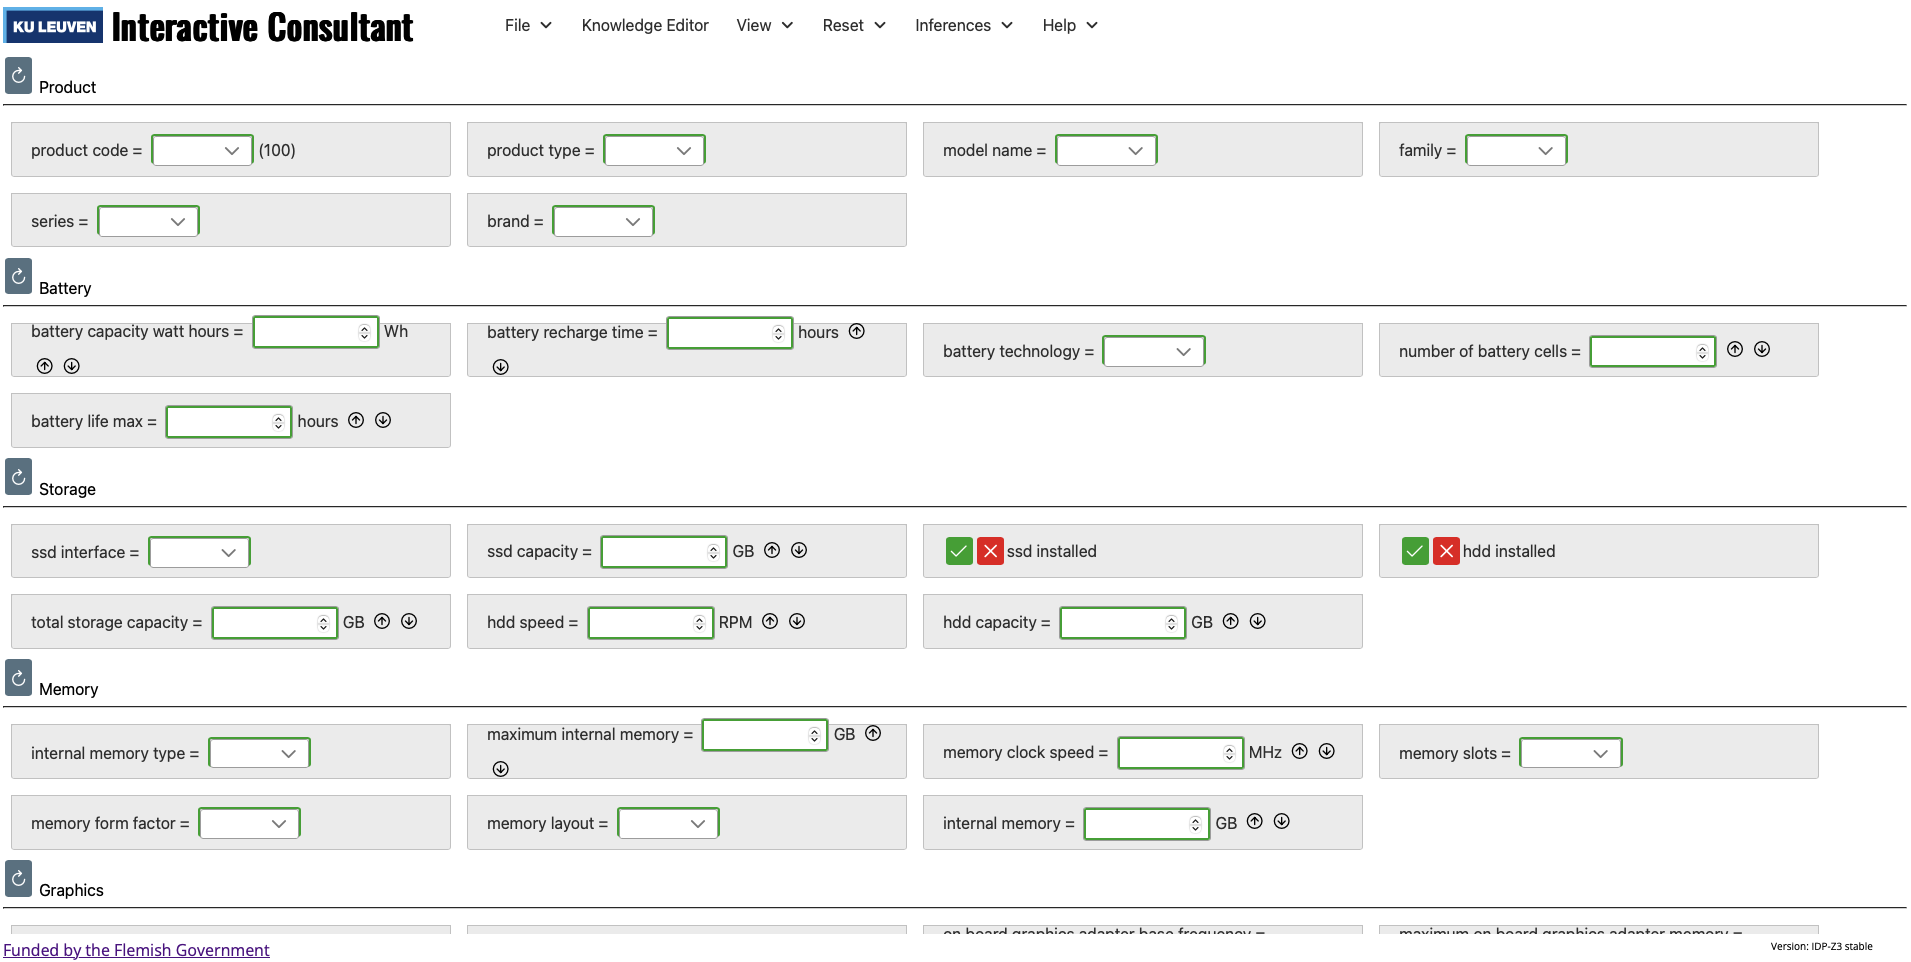
\includegraphics[width=1\textwidth]{gui.png}
    \caption[Huidige gebruikersinterface.]{\label{fig:gui}De online shop voor laptops in de Interactive Consultant~\autocite{KULeuven}.}
\end{figure}

\subsection{Frontend - GUI}
Voor dit onderzoek wordt er gekeken naar de grafische gebruikersinterface van een online shop voor laptops. De grafische user interface is uitgewerkt in Angular, een TypeScript-based open-source front-end framework dat ontwikkeld is door Google. Er wordt gebruik gemaakt van de PrimeNG UI-componentenbibliotheek. Deze library biedt een verzameling van herbruikbare componenten.

\subsubsection{Opbouw GUI}
\paragraph{Header}
De header bevat het KU Leuven-logo, een titel en een menubalk, en blijft behouden in de nieuwe UI (zie Figuur \ref{fig:header}).

\begin{figure}
  \centering
  
\includegraphics[width=1\textwidth]{header.png}
  \caption[Header huidige en nieuwe UI.]{\label{fig:header}De header van de Interactive Consultant met alle componenten~\autocite{KULeuven}.}
\end{figure}

\paragraph{ScrollPanel}
De content van de pagina zit vervat in een ScrollPanel. Deze scrollcontainer is opgedeeld in rijachtige structuur voor elke categorie van properties (zie Figuur \ref{fig:scrollpanel}).

\begin{figure}
    \centering
    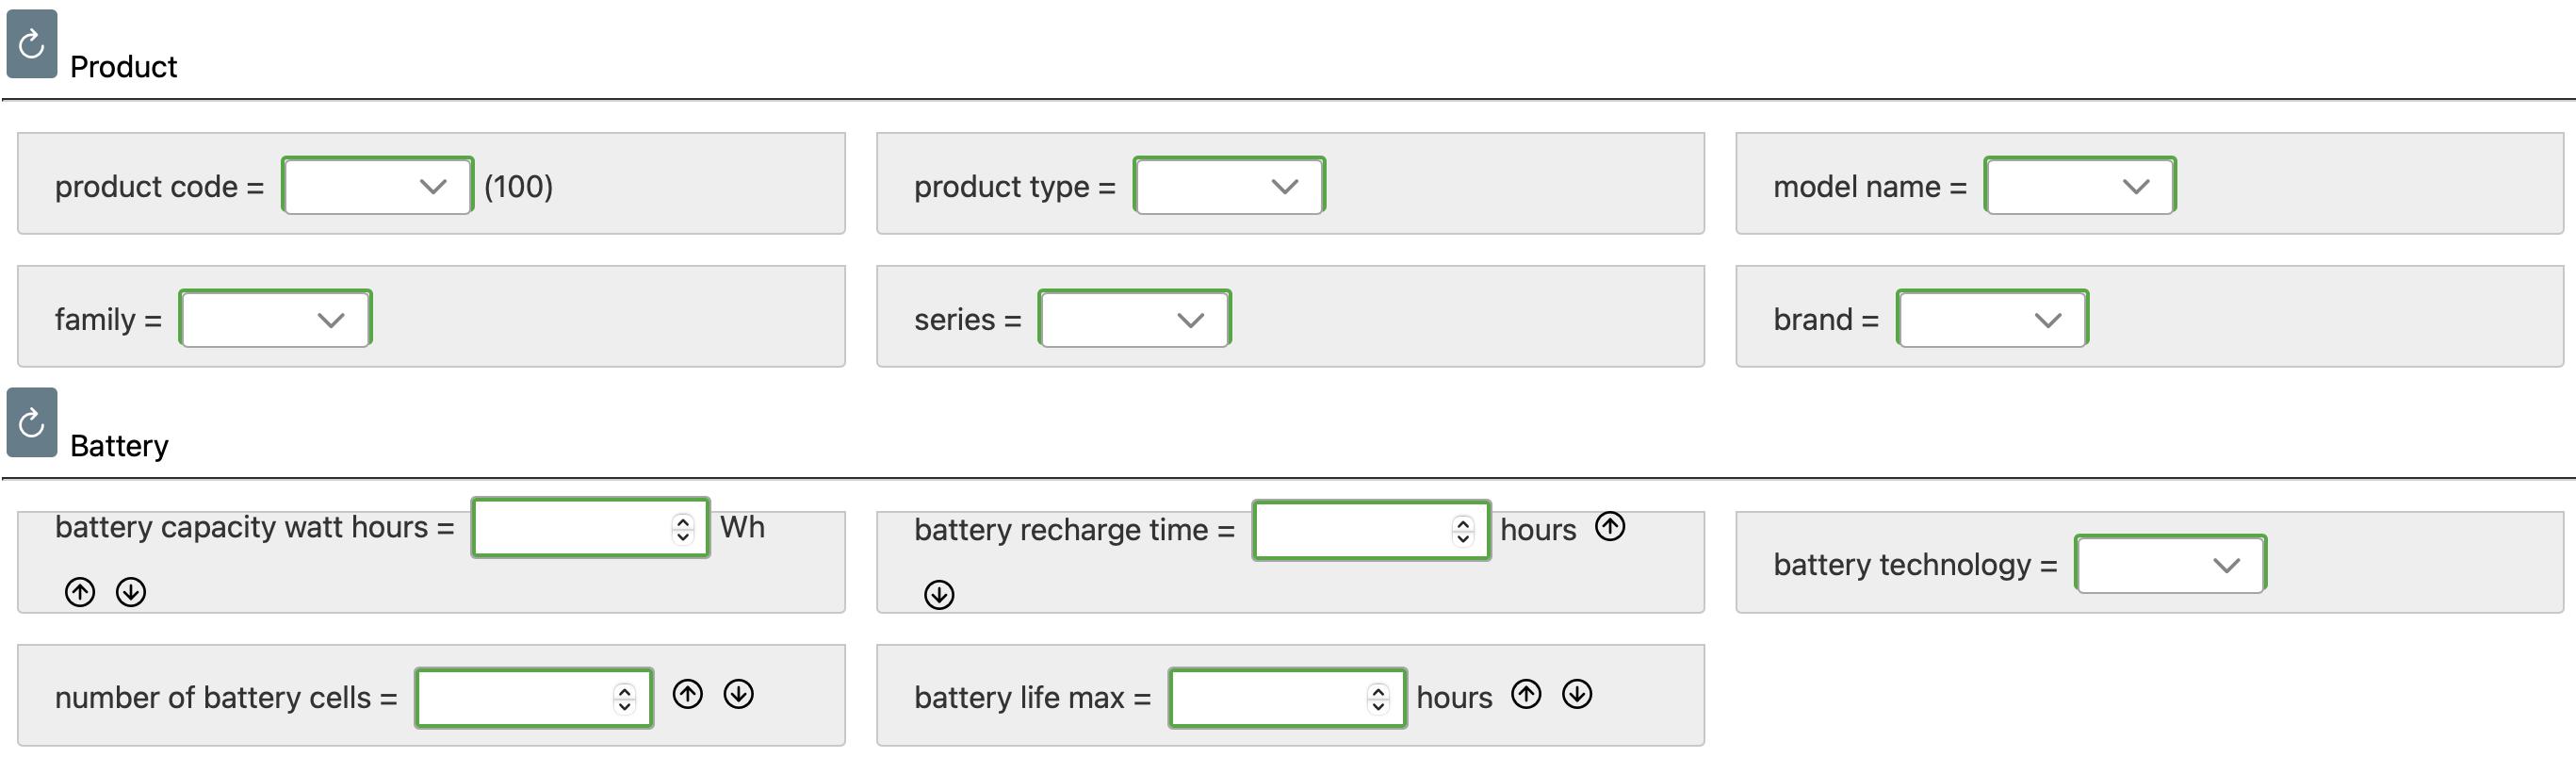
\includegraphics[width=1\textwidth]{scrollpanel.png}
    \caption[ScrollPanel van huidige UI]{\label{fig:scrollpanel}De content van de ScrollPanel opgedeeld in rijen op basis van de categorie van een property. In bovenstaande afbeelding zijn properties uit categorieën \textit{Product} en \textit{Battery} te zien~\autocite{KULeuven}.}
\end{figure}

\paragraph{Dropdown, binaire keuzeselector en invoerveld}
De properties worden weergegeven als dropdowns, binaire keuzeselectoren of invoervelden, afhankelijk van het type keuze dat de gebruiker moet maken. Dropdowns worden gebruikt wanneer er meerdere opties beschikbaar zijn, terwijl binaire keuzeselectoren geschikt zijn voor beslissingen met slechts twee mogelijke waarden, zoals ja/nee of aan/uit. De invoervelden zijn van het type number, waarbij zowel gehele als decimale waarden kunnen worden ingevoerd. In figuur \ref{fig:componenten} worden de drie UI-componenten afgebeeld.

\begin{figure}
    \centering
    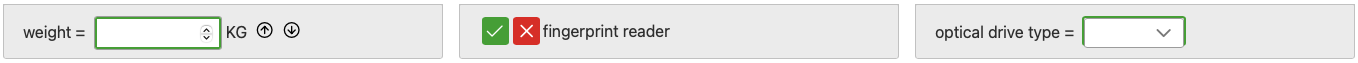
\includegraphics[width=1\textwidth]{componenten.png}
    \caption[Dropdown, binaire keuzeselector en invoerveld]{\label{fig:componenten}Voor property \textit{weight} wordt  een numeriek invoerveld gebruikt, terwijl voor property \textit{fingerprint reader} een binaire keuzeselector wordt toegepast. De property \textit{optical drive type} wordt voorgesteld met een dropdown~\autocite{KULeuven}.}
\end{figure}

\subsection{Backend - Technisch}
\subsubsection{IDP-Z3}
%Bron: https://docs.idp-z3.be/en/latest/introduction.html
IDP-Z3 is een redeneersysteem dat het Knowledge Base-paradigma implementeert met behulp van de FO[·]-taal. FO[·], ook bekend als FO-dot, is Eerste-Orde Logica waarmee kennis over een specifiek probleemgebied wordt vastgelegd. Deze kennis wordt vervolgens gebruikt om die problemen op te lossen door middel van redeneringen~\autocite{Carbonnelle2024}. Meer informatie over IDP-Z3 en de werking ervan is terug te vinden in de documentatie van~\textcite{Carbonnelle2024}.

\subsubsection{Properties}
De properties worden ingeladen met een JSON-bericht. Wanneer een gebruiker een wijziging aanbrengt in een veld, wordt het systeem opnieuw berekend en wo\-rdt er een nieuw JSON-bestand naar de IC gestuurd. De IC communiceert continu met IDP-Z3 om tot een oplossing te komen.

\subsubsection{Datamodel}
Er is geen persistente opslag van de ingevoerde gegevens, wat betekent dat deze niet bewaard blijven tussen sessies of voor toekomstige gebruik. Omdat de backend alles opnieuw berekent, is er geen sprake van een klassiek datamodel waarin gegevens kunnen worden opgeslagen en later opgehaald. Dit maakt het systeem flexibel en zorgt ervoor dat het altijd met de meest actuele gegevens werkt, maar betekent ook dat er geen historisch overzicht of hergebruik van gegevens mogelijk is. Dit laatste aspect is van cruciaal belang voor de nieuwe gebruikersinterface.

\section{Requirements-analysefase}
Bij het ontwikkelen van een nieuwe gebruikersinterface is het belangrijk te weten waaraan deze moet voldoen. Hiervoor worden zowel de functionele als niet-functionele vereisten geformuleerd. Daarnaast worden ze geordend volgens prioriteit, gebruik makend van de MoSCoW-methode. Deze fase kan beschouwd worden als de start van de vergelijken\-de studie van beschikbare technologieën en bibliotheken.

\subsection{Functionele vereisten}
Deze vereisten beschrijven de functionaliteit die het systeem moet bieden, oftewel de functies die de interface moet ondersteunen om de gebruiker te helpen.

\subsubsection{Selecteren van properties}
Een gebruiker moet op properties kunnen klikken om een waarde in te vullen voor de gekozen property of om de verklaring te krijgen waarom een waarde al is gekozen of ingevuld.

\subsubsection{Geselecteerde properties bijhouden}
De geselecteerde properties moeten worden bijgehouden en apart weergegeven.

\subsubsection{Deselecteren van properties}
Een gebruiker moet eerder gemaakte keuzes, zowel door zichzelf als door het systeem, ongedaan kunnen maken door een property te deselecteren. De waarde van de property moet worden gereset, zodat de betreffende property niet meer wordt bijgehouden of greyed out is.

\subsubsection{Resetten van properties}
Een gebruiker moet de waarden van alle properties kunnen resetten.

\subsubsection{Hoveren over properties}
Een gebruiker moet over properties kunnen hoveren om meer uitleg te krijgen over wat de betreffende property inhoudt.

\subsubsection{Real-time feedback}
De interface moet de gevolgen van de selecties van een gebruiker weergeven en moet kunnen verduidelijken waarom bepaalde keuzes automatisch worden toegepast. Een gebruiker moet dus directe feedback krijgen voor elke keuze die hij maakt.

\subsubsection{Opslaan klikgedrag en visuele indicaties}
Het systeem moet bijhouden welke properties door gebruikers worden aangeklikt, samen met de bijhorende relevantie. Wanneer een gebruiker een keuze ongedaan maakt door een property te deselecteren, moet het systeem de relevantie van die property opnieuw aanpassen. Op basis van deze relevantie bepaalt het systeem een gewicht of grootte voor elke property. Properties die frequent worden aangeklikt, worden groter en opvallender weergegeven. Het systeem werkt de weergave van de properties dagelijks bij.
\subsubsection{Begeleiding}
De opgeslagen informatie van de properties wordt gebruikt om gerichte aanbevelingen te doen aan gebruikers. De interface moet vrijblijvende hulp en begeleiding bieden zonder de vrijheid van de gebruiker te beperken. Dit is belangrijk, aangezien de huidige interface geen ondersteuning biedt.

\subsubsection{Visuele hiërarchie en uitlijning}
De interface moet een duidelijke visuele hiërarchie en uitlijning hebben, met een logische structuur voor de presentatie van gegevens, zodat de gebruiker niet wordt overrompeld door te veel informatie. Dit is essentieel, omdat dit momenteel het probleem is van de bestaande gebruikersinterface.

\subsubsection{Eenvoudige navigatie}
De interface moet een eenvoudig navigatiepad bieden, zodat een gebruiker snel de gewenste informatie kan vinden en te allen tijde weet waar hij zich binnen de interface bevindt.

\subsubsection{Backend integratie met IDP-Z3}
Het systeem moet in staat zijn om te communiceren met IDP-Z3, wat momenteel gebeurt op bais JSON-berichten. Deze werkwijze moet behouden blijven. 

\subsection{Niet-functionele vereisten}
Deze vereisten beschrijven hoe het systeem de functionele vereisten moet uitvoeren. 

\subsubsection{Gebruiksvriendelijkheid}
De interface moet gebruiksvriendelijk zijn, zonder onnodige complexiteit en intuïtief aanvoelen, zodat een gebruiker er vlot mee kan werken.

\subsubsection{Prestaties}
De interface moet snel reageren op gebruikersinvoer en zonder merkbare vertraging worden bijgewerkt.

\subsubsection{Esthetiek en visueel design}
De interface moet een aantrekkelijke visuele laag bieden die de gebruiker niet alleen ondersteunt, maar ook een aangename ervaring biedt. Het design moet consistent, responsive en modern zijn.

\subsubsection{Gebruik van kleuren}
De interface gebruikt kleuren om aan te geven welke properties relevant zijn en welke niet.

\section {Long list fase}
Aan de hand van deze eisen en de informatie verzameld in de vorige fasen, zullen er potentiële front-end softwarebibliotheken worden gezocht en opgesomd. Hiervoor wordt de literatuur opnieuw geraadpleegd.

\section {Short list fase}
Vervolgens wordt de lijst met alle gevonden alternatieven uitgedund. Via een samenvattende tabel worden de meest geschikte front-end softwarebibliotheek geselecteerd.

\section{Architectuur van de applicatie}
Een softwarebibliotheek is niet voldoende om een webapplicatie te bouwen. De architectuur van de applicatie moet ook uitgetekend en besproken worden. Er zal bepaald worden welke technologieën de applicatie moet bevatten. Hieronder is een hypothetische opstelling omtrent de architectuur van de applicatie gegeven:

\begin{itemize} 
    \item \textbf{Frontend:} Dit framework zal afhangen van de gekozen front-end softwarebibliotheek. Deze moeten namelijk compatibel zijn.
    \item \textbf{Backend:} Dit framework zal afhangen van het gekozen front-end framework. Deze m\-oeten met elkaar kunnen communiceren. Er zal gebruik gemaakt worden van een REST API-server.
    \item \textbf{Database:} Voor het bepalen van et datamodel en de databank kan er gekeken worden naar de huidige technologieën, maar dit is niet noodzakelijk.
\end{itemize}

\section{Proof-of-concept bouwen}
Nadat alle technische keuzes gemaakt zijn, zu\-llen deze getest en uitgewerkt worden. Er zal een prototype gebouwd worden om te valideren dat de gekozen technologieën effectief werken en de problemen oplossen.

\section{Conclusiefase}
Na de proof-of-concept wordt er een aanbeveling gegeven over het beste mogelijke alternatief. Ook de overgebleven  aspecten die niet aanwezig zijn in een van de onderzochte opties worden geïdentificeerd.